% 来源：OEBPS/Text/Section0001_split_003.xhtml#sigil_toc_id_25

\BookChapter{15}
\section[第15章\q 梦想的价码是多少？让游戏能赢]{第15章\\ 梦想的价码是多少？让游戏能赢}

\begin{BookQuote}
人人都有梦想，但人和人的梦想不大一样。

\hfill ——T. E. 劳伦斯
\end{BookQuote}

我举办投资理财研讨会，开场总是用下面这个问题：“你梦想的价码是多少？”接着我会邀请参会的人站起来，告诉我，需要多少钱，才能让他们实现财务安全、财务独立、财务自由。大多数人都一头雾水，根本不知道如何回答。有人支支吾吾，有人扭来扭去，之后可能会有几个人举起手来。我主讲过几百次研讨会，有来自各行各业的成千上万的人，我听到过各种各样的财富目标数字。你能想象到的数字，我都听说过。

现在我来问你，你自己想想看，你需要多少钱才可以实现财务安全、财务独立，甚至财务自由？不需要精确的数字，甚至不需要合乎逻辑。100万美元？500万美元？5000万美元？现在只用1秒钟，只用你的直觉，写下你感觉到的数字，就写在本书的书页边上，写在手机上，或者随便找片纸，只要写下来就行。最重要的是写下来这个动作，写下来就相当于定下来了，你会感觉这个数字特别真实。

你写好了吗？很快你就会明白，为什么写下来这一步是非常重要的第一个行动。

现在，我的经验告诉我，你如果像大多数人一样，你就会感觉自己写的那个数字对于自己来说有点太大了，是不是？好，接着读下去，因为我们将会做一些非常轻松的练习来帮助你征服这个数字。我敢打赌，这会让你发现，你能让这个数字看起来很小，比你想象到的还要小得多。事实上，你将学会不仅只有一个“魔术数字”，因为你会有五个不同水平的财务梦想，让你实现自由。不管你是刚刚开始工作还是准备退休，不管你的财务收支非常稳固还是摇摇欲坠，我敢保证，这五大梦想中至少有两个都在你的能力范围之内，都是你能够实现的。怎么实现？你首先要了解你真正的需要是什么。

最近，我的高端课程上有个年轻人，他坐在房间后面，站了起来，大声说出了他的梦想的价码。他抬头挺胸地高声说道：“10亿美元。”

人群中响起了一片“噢”“啊”的惊叹声。这个人有20多岁，在参加这次会议的人里面，他算是很年轻的，他可能还没有挣到他人生的第一个100万美元。于是我就让他考虑下，这个数字的真正意义。

我们在第4章中讲过，人们做的每一件事的背后都有一个理由。简单提示一下，人们有六个基本的人类需要：确定性，不确定性/变化，重要性，联系/爱，成长，奉献。为什么这个年轻人想要得到10亿美元？他想要满足的是六大基本需要中的哪一个需要？你可以在生活中得到确定性，需要的钱远远少于10亿美元！你可以得到足够的变化性，用100万美元就行，甚至再少很多也行，对不对？联系和爱呢？这事很难。就算这个小伙子得到了10亿美元，那么肯定会有很多人想要进入他的生活，就像买彩票中了大奖一样，你发现一下子冒出来几十个亲戚和“朋友”，可是自己以前根本不认识他们。有了这么多钱，这个小伙子肯定可以得到联系，但是这并不是他想要的和他需要的。成长和奉献呢？从他的言行举止来看，我觉得他报出了10亿美元这个数字的时候，成长和奉献并没有排在他的需要清单的首位。

你个人认为哪一个需要对这个小伙子的驱动力最强？很明显是重要性。正如他所说的，有了10亿美元，人们就会非常尊重他。他这个10亿富豪对于人们来说很重要，这也许是真的。但问题是他就算有了10亿美元，也是不够的，因为你追求的是重要性，你总会把自己和别人比较。人外有人，天外有天，总会有人比你更高、更强、更快、更富、更有趣、更年轻、更帅、更美，总会有人比你的游艇更大、车子更酷、住宅更豪华。所以重要性本身没有错，但如果你把它当作第一大需要，你就很难得到完全的满足。

但是我并没有教育这个小伙子，我决定展示给他看，让他明白要感觉到自己很重要，只用远远少于10亿美元的钱就可以做到——大幅降低目标，会让他的日子过得更容易。公开说自己需要10亿美元，让他感觉自己在追逐很大的目标。但问题是，把这么巨大的目标装进脑袋，而你的直觉和你的本能并不相信这个目标真能实现，你的大脑就会排斥这个目标。你就会像为了一个谎言而活着。你做过这样的事情吗？编织出一个巨大的目标，脑袋里蹦出一个声音说道：“你开什么玩笑！”真相是你永远不能实现你的目标，直到你让这个目标深深地沉入你的潜意识——潜意识是你大脑中最强大的那个部分，是它让你的心脏每天跳动10万次，而你根本想都不用想心跳这回事儿。

当开着车的时候，你一下子走神儿了，陷入了某种思绪，突然一下子醒悟过来，才意识到自己走神儿了。你是否有过这样的体验？“我的天哪，前面这5分钟是谁在开车啊？！”感谢神力无边的人生保护神——你的大脑潜意识。

要了解这种过程是如何进行的，可以看下面的这张图。想象你的大脑被分成了上半区和下半区，上半区是有意识思考，下半区是无意识思考，即潜意识。

\begin{figure}[htbp]
\centering
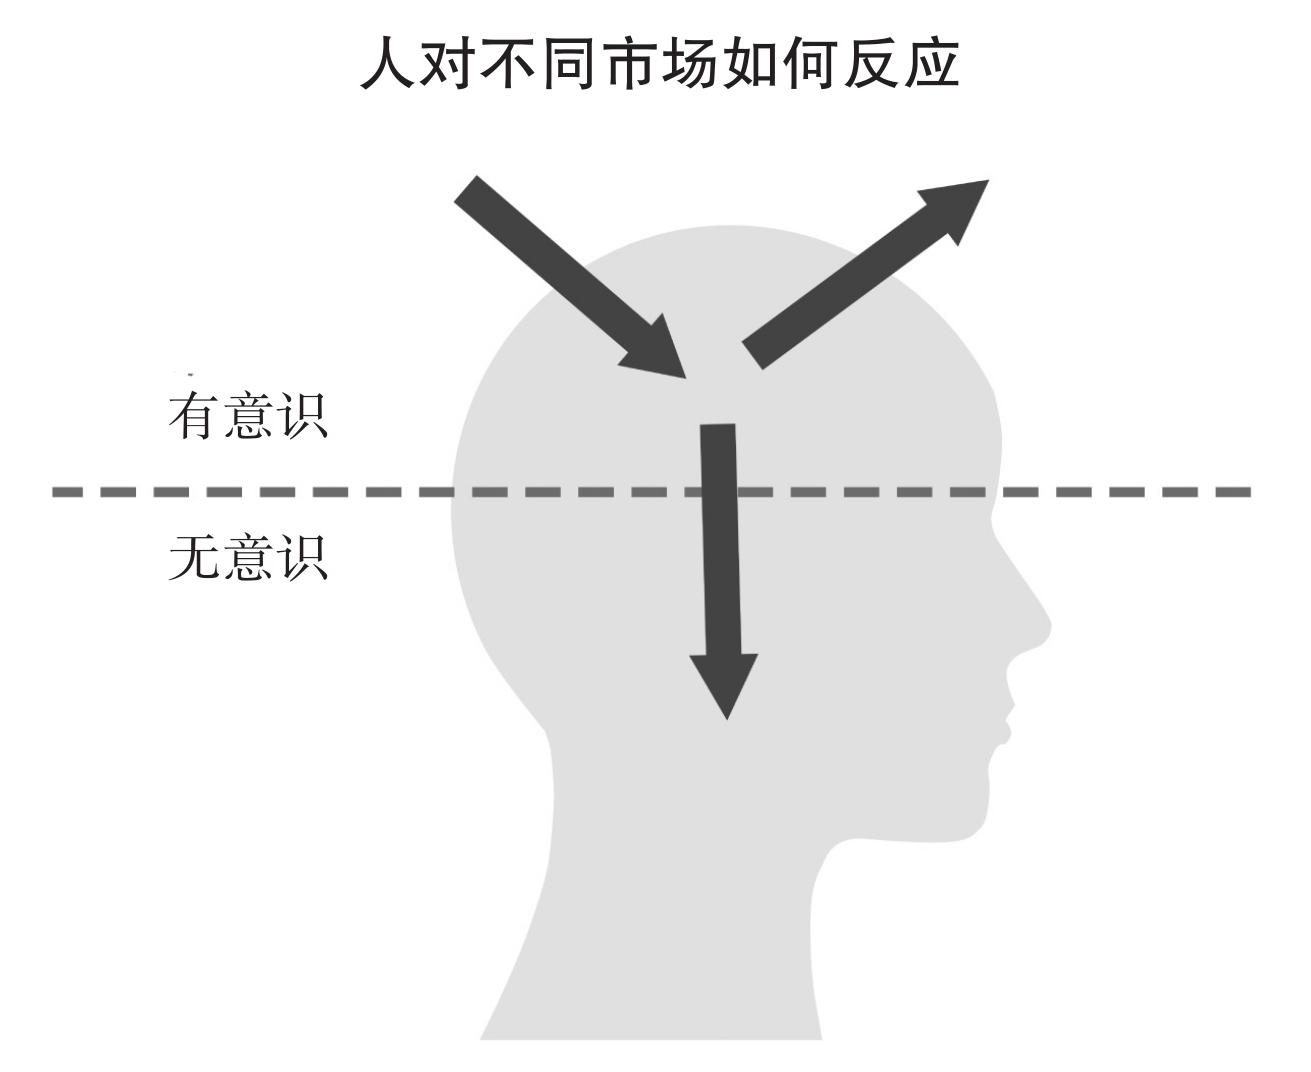
\includegraphics[width=0.68\linewidth,keepaspectratio]{image/15-1.jpg}
\caption{}\label{fig:15-1}
\end{figure}

各种各样的想法不停地想要进入你的大脑，比如，“我想赚1000万美元”“我想40岁实现财务自由”。但是你的大脑上半区，就是有意识的大脑部分会说：“去你的！这种事情根本就不可能发生！”有意识的部分很快拒绝了这样的想法进入意识，把它反弹回去了，就像一个网球一样，从哪里来再回到哪里去。但是如果你下定决心，有着非常确定的感觉“我要做成这件事”，接下来，你就开始构建一个计划，某件神奇的事情就发生了。你开始逐步形成确定性：你真的能够实现这个愿望。有了新找到的自信，你会突然看见，其实有个办法可以做成这件事。你会找到一个榜样，这个人已经实现了你在追逐的目标，你只要跟着他的成功方法一步一步地做就行了。你会开展大量的行动。这个目标深深地沉入你的潜意识中。这样你的潜意识就开始工作了，它让你的梦想变成现实。这个时候就是奇迹发生的时候。

现在我怀疑，你是不是还认为你需要10亿美元来实现你的财务梦想。但是我愿意打个赌，你选择的能让你感到财务安全和财务独立的那个财富数字，肯定会大得吓人。几乎每个人说出的那个财富数字，都远远大于他们实际所需要的财富数字。因为他们并没有花时间计算，用一种和他现在完全不同的生活方式来生活，到底需要花多少钱。也正是因为这个原因，很多人从来没有开始朝这个目标努力行动。他们只是口头上说说而已，大脑想到这么大的财富目标自然会很激动，跟别人一说自己有个这么大的梦想，听起来也很有面子，但他们从来没有开始付诸行动，为实现这个目标努力奋斗。因为从内心来讲，他们根本没有把握自己肯定能够做到这一点。而这种确定性是人类的第一大需要，会影响我们的行为和行动。事实正是如此。如果你没能采取行动来改变你的财务状况，一部分原因是你不能确定什么是对的，什么是错的，不能确定哪条路会成功，哪条路会失败。你感觉整个人完全不知所措，因为整套做法太复杂了，没有人愿意花时间来教你，让你看得清清楚楚。由于存在不确定性，我们一般会干脆什么也不做，或者起码会一拖再拖。本来今天需要做的事，我们会拖到明天再说。

为了帮助我那些未来的亿万富翁朋友，确认他们梦想的真正价码，让他们可以把这个数字固定到他的潜意识里，然后梦想成真，我问了他们一些问题。我很快就会问你同样的问题，来指导你走好你的财富自由之路。

我先问这位年轻的朋友，当有了10亿美元的财富后，你的生活会是什么样子的。他想了一会儿才说：“我要拥有自己的湾流私人飞机（世界上最快、最豪华的公务飞机）。”

“你自己的私人飞机！”我说，“你要飞到哪里？”

他说：“哦，我住在纽约，或许我想飞到巴哈马。我也可能飞到洛杉矶，去参加一些会议。”

我让他写下来他一年大概会飞多少次。他估计一年最多飞12次，那么一架私人飞机要花掉他多少钱？我们查了一下，一个飞行距离最长的湾流G650机型会花费他6500万美元，要是买一个二手湾流IV机型，可以让他节省1000万美元。这些费用并不包括燃油费、维护保养费、机组人员的工资费用。接下来，我们又查了一下，自己不拥有，而是租用一架私人飞机的成本：一个中型的私人飞机，足够满足他自己加上三个家庭成员的飞行需要了，租金大约是每小时2500美元。这个小伙子也许每年要飞行100个小时，总共每年的租金支出需要25万美元；即使每小时的租金为5000美元，他每年的租金成本合计也只需要50万美元——远远低于很多私人飞机的年度保养费用。即使是如此豪华的湾流私人飞机，其每年的租金成本也低于购买成本的1\%。尽管我站在舞台上，和那个小伙子隔得很远，我也能看到他的双眼放光，很明显他的脑子在快速运转。

“你有10亿美元，除了私人飞机，你还想买什么？”我问他。

“一座私人小岛。”

这事巧了，正好我也有经验。因为我在斐济这个小国拥有一座人间天堂般的小岛。我在很年轻时，就有一个狂野的梦想，想要找到一个世外桃源，有一天，我带着我的家人和朋友可以到那里生活。我20多岁的时候，游遍了全世界的海岛，想要找到我的香格里拉。后来我来到了斐济，我找到了。这个小岛不但有魔幻般的美景，而且有美丽的灵魂，可是那个时候我的钱不够多，不能买下整个小岛，但是我在这个小岛上买了一个小型背包客度假胜地，面积有125英亩\footnote{\label{fn:pdf-15-1}1英亩≈0.004平方千米。——编者注}。其实我当时没有多少钱，那时这也不是最好的投资。但是那是我“梦想水桶”的一部分，我在后面会给你详细讲述什么是梦想水桶。尽管如此，我还是办成了这件事。我可以骄傲地说，这些年来，我购买了它周围的更多土地，把这个度假胜地转变成一个生态保护区，它有500英亩的陆地，有接近3英里\footnote{\label{fn:pdf-15-2}1英里≈1.61千米。——编者注}的海岸线。我已经把马雷度假胜地和温泉浴场变成了最近十年斐济排名第一的度假胜地，而且持续位列南太平洋地区的十大度假胜地之一。但是我经常到这个天堂小岛去吗？由于我的日程被安排得繁忙到简直让人疯狂，一年能去那里4\textasciitilde{}6个星期就不错了，但是我的梦想成真了：每个到那里的朋友都过得非常开心。

我告诉这位年轻的朋友：“如果你想享受你自己的私人小岛，你也许应该进入酒店行业。相信我，你最多只会一年在那里待上几个星期而已。”我们查了一下成本发现，在巴哈马买一座岛屿只需要10万美元左右——之后他需要花费3000万\textasciitilde{}4000万美元建成一个小型的度假胜地。或者他可以租用我的朋友理查德·布兰森的内克尔岛度假胜地，租一个星期。他就算把所有的朋友和家人都请过来，费用也不会超过35万美元，而且他会有一个50人的团队来照顾你所有的客人。如果这个小伙子每年都来玩一个星期，持续十年，总共也只需要花费350万美元，和自己购买小岛并建成度假胜地所要花费的3000万\textasciitilde{}4000万美元的成本相比，它只占1/10，而且他根本不需要考虑维护保养这些设施。

我们分析了一遍他的梦想清单，估算了一下他接下来的人生如果按照这种生活方式度过的话，他实现梦想需要花费多少钱。你猜猜看。不仅是他的基本需要，还有他最狂野的梦想，实现他所有的人生梦想的实际成本不是10亿美元，不是5亿美元，也不是1亿美元，甚至不是5000万美元，而只需要1000万美元。只需要1000万美元，他就可以实现他的所有梦想，并按照他梦想的生活方式生活，而且根本不用去工作赚钱来维持这种生活方式——要知道他的梦想可是大得令人吃惊的。我们算出来的实际梦想总成本是1000万美元，和他想象的10亿美元的梦想总成本简直天差地别。这两个数字完全代表两个不同的宇宙。

问题和挑战是当我们碰到了一个真正非常大的数字时，人们的头脑好像无法弄清楚这个数字真正意味着什么。100万、10亿、1万亿，三者之间是千倍的差距，差别非常大。尽管奥巴马总统嘴里说起“百万”和“十亿”两个词所用的语气一样，好像它们有些相关性——其实根本不相关。我来证明给你看。我先来给你做一个小测试。我希望你先想一想，再试猜一下答案。这个练习能帮你正确认识，百万、十亿、万亿三个单位之间的差距究竟有多大。现在，美国政府官员好像一张嘴就是“万亿”，“万亿”成了新的“十亿”，他们现在说“万亿”的次数跟过去说“十亿”的次数一样多。

我的第一个问题是：100万秒前是多久之前？花一点时间想想看，尽管你可能并不知道答案——现在你猜猜看。

答案是12天之前！你的猜测跟答案差多少？不要感觉糟糕，大多数人都猜不对。如果你猜对了，祝贺你。现在我们要提高难度了，因为你现在对“100万”有点感觉了（100万秒相当于过了12天）。10亿秒之前相当于多久之前？跟着我，一起来猜。答案是32年前。你的猜测接近这个答案吗？对于大多数人来说，他们的猜测都跟答案差得很远。“100万”跟“10亿”之间的差别就是这么大：12天与32年。现在你明白了，为什么我说“100万”和“10亿”分别属于“不同的宇宙”了吧。你绝对不能用同样的语气说“100万”和“10亿”，说得好像它们是同样的数量一样。

接下来继续想一想：你听说美国政府的债务有17万亿美元的时候，是什么样的感受？请问1万亿是多少？好了，我来提示你一下，10亿秒相当于32年，那么1万亿秒相当于多长时间？答案是，近32000年（准确地说是31689年）！我的天哪，那时人类甚至还没有进化成人呢！这个练习的目的是让你意识到，我们的大脑经常弄不清楚大的数字究竟有多大，要是你能认真地看清事实真相，你会发现自己原来以为得到梦想中的非常奢华的生活方式需要很多钱，其实真正需要花的钱比想象的要少得多。

\begin{figure}[htbp]
\centering
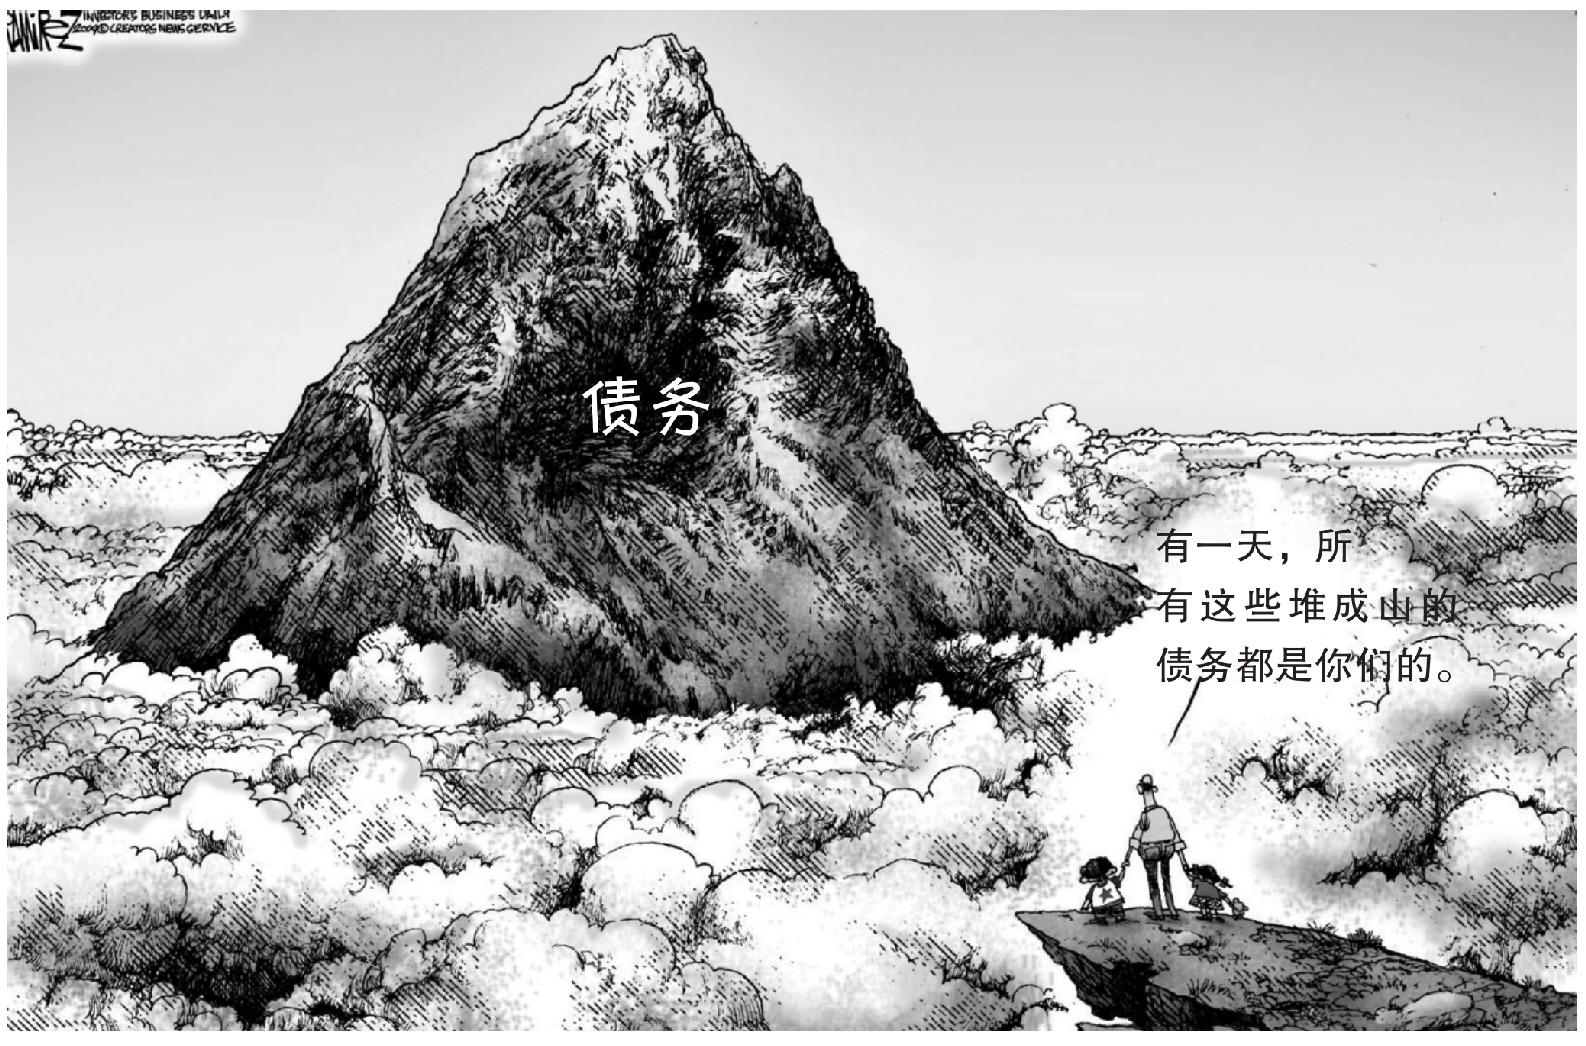
\includegraphics[width=0.75\linewidth,keepaspectratio]{image/15-2.jpg}
\caption{}\label{fig:15-2}
\end{figure}

现在回到我们那位未来想成为10亿美元富豪的小伙子。不过，请不要误解我的意思，1000万美元仍然是一个巨大的数字，但是现在这位年轻的企业家通过未来的努力，还是有可能赚到1000万美元的。谁知道？也许他最终也会赚到10亿美元——如果他发明了下一个Instagram的话。但是如果他没有赚到10亿美元呢？他仍然会过上他想要的豪华奢侈的生活，尽管他只赚到了1000万美元，比他认为自己过这种生活需要的10亿美元的财富目标少了99\%。他并不需要成为10亿富豪，也能享受到与10亿富豪一样奢华的生活品质。

我愿意跟你打赌，一旦你搞清楚了你的梦想的实际价码，那么你会发现，和你想象的实现自己梦想的生活方式所需要的财富水平相比，实际需要花的钱要少得多！你要记住终极真理：生活重要的不是钱，而是心情。真正的目标是拥有你想要的生活方式，而不是你想要的东西。你死了，你的这些东西都要被别人拿走。这些东西不会永远是你的，你生不带来，死不带去。我可不傻。尽管我非常珍爱和享受“我的”那个斐济小岛上的度假胜地，我心里很清楚，我只不过是个看管者而已。将来有一天会有另外一个人拥有这个产业。但是我非常高兴，我把这个地方培育成了一个旅游胜地，全世界的人都来这里游玩，体验到了快乐、浪漫、奇遇。这是我留给后人的一个遗产——拥有这样的成就，才是给予我快乐的原因。占有并不是目的，金钱本身并不是目的。我们个人的价值高低，并不能以银行账户里钱的多少来衡量，而应用我们灵魂的贵贱来衡量。赚钱的过程，钱能带我们去的地方，钱给我们带来的时间、自由、机会，这些才是我们真正应该追求的东西。

\begin{BookQuote}
你都能得到，只是不能一下子都得到。

\hfill ——奥普拉·温弗瑞
\end{BookQuote}

现在花些时间想想看，你用自己的钱真正想买的东西是什么。并不是每个人都希望自己过的生活像地产大亨特朗普\footnote{\label{fn:pdf-15-3}唐纳德·特朗普，2016年当选美国第45任总统。——编者注}或世界拳王梅威瑟一样！你的梦想是环游世界，探索古城，到坦桑尼亚的塞伦盖蒂大草原上给狮子拍照吗？你的梦想是拥有一套巴哈马的海边度假别墅，还是在纽约拥有一套顶层豪宅？你的梦想是创办自己的企业，编写下一个Snapchat（“阅后即焚”照片分享应用），还是为人类做出非凡的贡献，成为下一个“上善若水”公益机构？你的梦想是不是很简单，攒的钱能送孩子上大学，还能剩下来足够的钱在郊区买个别墅，有个大花园可以种花、种草、种菜？或者你的梦想只是想得到内心的安宁——你知道你永远摆脱了债务和担忧呢？不管你的梦想是什么，我都会给你指出一条实现梦想的道路。即使你可能不能走完全程到达顶峰，你也可以实现那些对你来说最重要的梦想，一路上不断地庆祝自己实现了一个又一个梦想。因为钱是一个情绪的游戏，我们会提出一些数字，让你一看就信心十足。你马上会说：“我肯定能行！我敢向自己保证我能做到！”

像所有的旅程一样，开始上路之前，你需要弄清楚自己现在在哪里。我们一起来做几个简单的计算。如果你从来没有花时间想清楚实现自己的财务目标需要多少钱，没关系，你并不孤独。情况常常是，很多赚到百万美元的人还没有制订出一个计划，以保持现在的生活方式，让自己不用为此而靠工作赚钱，至少有一段时间可以不用工作。正如我们前面所说过的，超过一半的美国人从来没有试着算一算，自己需要攒多少钱才能安享退休生活，其中包括美国46\%的投资理财规划师！为什么我们会不知道自己的基本财务情况？我听过上百个国家成千上万人的回答，我发现，第一大原因是心里害怕，不敢知道。

这就好像很多人不愿意踏上称重器一样。你知道自己的体重超标，但是你就是不想知道自己有多重。其实这既是一种拒绝承认现实的表现，也是一种拖延着不去改变自己的办法。摔跤选手和职业拳击手每天都会踩上称重器，这样如果体重超标，他们自己会马上知道，以便采取行动及时减重。你不测量体重，就不能管理体重。你不做身体检查，就不能管理身体健康。同样的道理，你不检查你的财务状况，就不能管理你的财务。你只有知道要实现你的财务梦想需要多少钱，才能有机会实现你的财务梦想。我是来帮助你的，让你脱离愚昧。大部分人一谈到自己有多少钱、需要多少钱，就像鸵鸟把头埋进沙子里一样不管不顾。只用1分钟，我们来做一些简单、快速的数字计算，以便弄清楚你现在的财富处于什么水平，以及你需要达到什么样的水平。

不过，我们先来看看这五大财务梦想：财务安全、财务活力、财务独立、财务自由、绝对财务自由。这五大财务梦想，你听起来是不是感觉好像一回事？你大声地说出来，它们是不是分别带给你不同的感觉？试试看。哪个使你感觉更高一级？安全还是活力，活力还是独立，独立还是自由，自由还是绝对自由？这五个财务梦想逐级加大，是不是？实现不同财务梦想的财富数字也会不同。

在这五个梦想里，你也许发现自己只是致力于实现其中一两个梦想。对于有些人来说，财务安全这一个梦想就能改变人生，给他们巨大的自由。因此，设计这个练习的时候，我把这五个梦想分成5步，一路走下来，通往绝对财务自由。或者换个比喻，你还记得本书前面提到的那座山吗？你就像登山一样，从山底的大本营一路攀登到顶峰。记住，并不是我们每个人都需要爬完全程到达珠穆朗玛峰峰顶。对于有些人来说，能实现财务活力的梦想就是享大福了，要是能够实现财务独立就像到天堂了！并不是这五个梦想对于每个人来说都是“必须的”。

我请你好好读读这五个梦想，从中选出三个对你最重要的梦想，我称之为“三生万物”。你会拥有三个目标：短期目标、中期目标、长期目标。这样设置目标是因为，我们不能在失败的基础上打造成功，我们只能在成功的基础上不断地打造梦想。你如果只是为了长期的一个大数字而努力，可能会感觉太远，甚至会觉得数字大得让人害怕，结果你可能从来不会真正开启这段旅程。我们需要一个目标，既足够近，让我们觉得肯定能够达到那里，又在相对比较近的未来，这会让你采取行动，把一个短期目标变成现实。记住一路上要不断地宣扬你的胜利。为什么要在你实现财务独立了之后，才去庆祝？为什么不在每个阶段都获胜，然后一个阶段接一个阶段地庆祝？这样做可以持续鼓励你，刺激你，给你前进的动力。

\begin{BookQuote}
需要多大的能量计划，就需要多大的能量盼望。

\hfill ——埃莉诺·罗斯福
\end{BookQuote}

\subsection{第一个梦想：财务安全}

安全意味着什么？不是我来告诉你，而是要你自己想，所以我们换个方式。我来问你：“如果下面五样东西的开支都付清了，你的余生再不用靠工作而赚钱，你会感觉有多了不起呢？”

1.你房子的抵押贷款还清了。这辈子你再也不用靠工作来赚钱还房贷了。

2.你未来的公用事业费全部付清了。你再也不用靠工作赚钱交水费、电费和电话费了。

3.你家里人未来所需的所有食物的费用全部付清了。

4.你未来的基本交通费用全部付清了。

5.你未来的基本保险费全部付清了。

我打赌，你的生活品质将会让你感到非常满意，是不是？你感觉非常安全，因为你知道所有这些东西的费用都有保障了。

现在还有一些好消息：记住你前面写下来的那个数字——你觉得能让自己实现财务安全和财务自由的财富数字。可能你并不像我前面说的那个小伙子那么极端，认为需要赚到10亿美元才够花，这个数字也太大了，但是你想的那个财富数字自己还是感觉相当大的，对不对？没关系，我敢打赌，在你真正搞清楚这个数字后，它会让你非常吃惊，财务安全的梦想可能比你想象的要近得多。如果你是极少数过分低估财务梦想所需要的财富数字的人，你需要做个现实情况核查，让自己知道实现你的财务梦想所需要花的钱的精确数字是多少。

你如果还没有下载我们的免费App，现在赶紧下载，或者用下面的工作表，写下你这五个开支项目每个月花的钱。其实很简单：第一项，你现在的房地产抵押贷款的月供。（你如果现在还很年轻，还没有自己的房子，那就写下来你每个月的房租。你可以估计一下或者到网上查一下，可能不是买一套你理想的房子，而是先买一套实用的房子就行。）你大概每个月要还多少房贷，你如果有过去的历史账单记录，就很容易了，查一下就行。第二项，你每个月的公用事业账单和电话费。第三项，你每个月花在吃饭上的钱。……就这样一项一项地来，你如果手头找不到花销的数据，大概估计一个就行——你随时可以修改，但是你不能失去干这件事的冲劲。我们就是要实实在在地算出来一个合理的数字。查查你的银行账户或者上网查一查，找到需要写下来的这五项开支的数字。保持你现在的这种冲劲，不要让它凉下来。我来给你一个样板。

\begin{figure}[htbp]
\centering
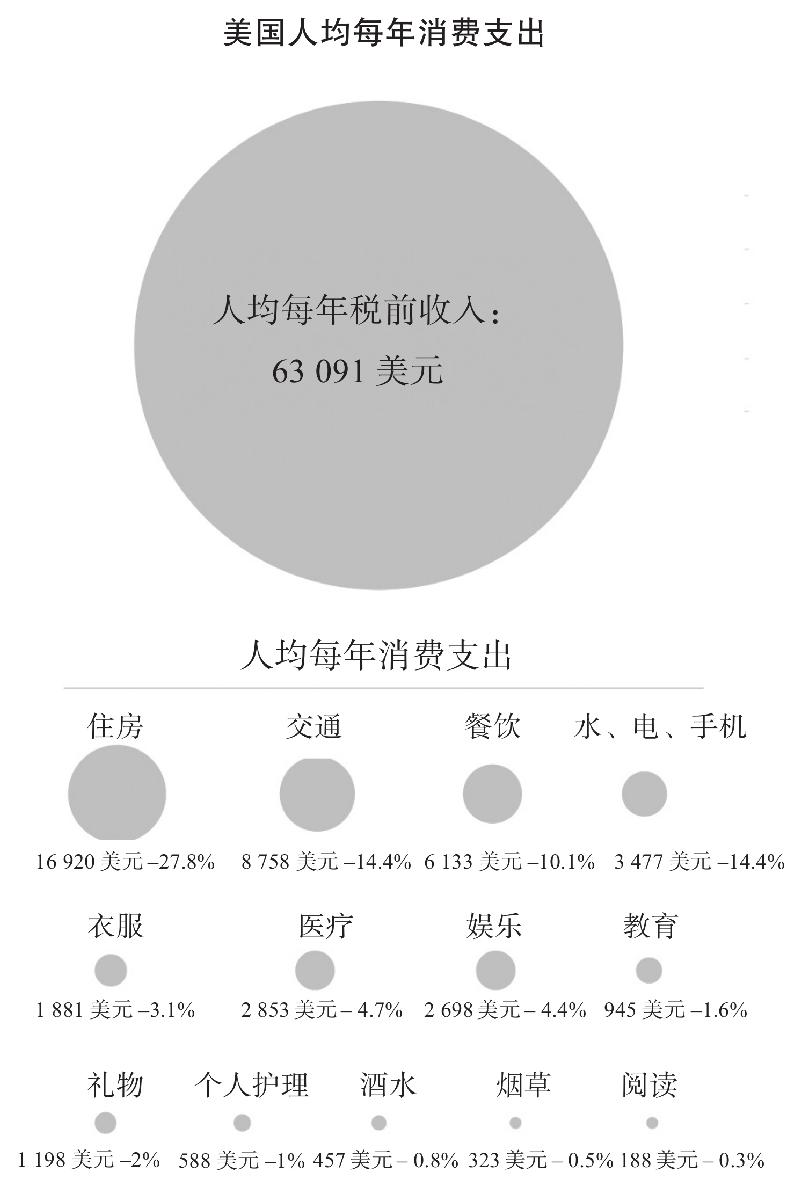
\includegraphics[width=0.74\linewidth,keepaspectratio]{image/15-3.jpg}
\caption{}\label{fig:15-3}
\end{figure}

你还记得我的朋友安吉拉吗？我在第一章给你讲过她。她48岁，单身。她想弄清楚，她要达到财务安全，究竟需要多少钱。她一开始猜需要300万美元。这个数字正确吗？是不是差不多？我让她做了一遍这个练习，写下她每个月的上述五项基本开支。结果表明，她的数字几乎和美国全国平均水平一模一样，你一看下面的列表就能看出来。

1.房租或者房贷：每月\_\_\_\_美元（安吉拉平均：1060美元）

2.食物，日用品：每月\_\_\_\_美元（安吉拉平均：511美元）

3.水费、电费、天然气费、电话费：每月\_\_\_\_美元（安吉拉平均：289美元）

4.交通：每月\_\_\_\_美元（安吉拉平均：729美元）

5.保险：每月\_\_\_\_美元（安吉拉平均：300美元）

6.合计：每月\_\_\_\_美元（安吉拉平均：2889美元）

7.美国人均年度基本开支：每年\_\_\_\_美元（平均为34688美元）

她把表格填完了，我让她把这五项基本开支加到一起，由此得到每月的基本开支，再乘以12，这就是她覆盖五项基本开支所需要的年收入水平——不用工作就有这么多收入。这就是财务安全，你可以看到她的每年基本开支是3.4万美元，和美国平均水平基本相当。

现在，安吉拉怎么做才能每年不用工作就能拿到3.4万美元的收入？记住，她要打造一个赚钱机器，她的工资收入有10\%会自动储蓄起来。她把这些钱转入了罗斯401(k)账户，这些钱会被投资到收费很低的指数基金上，预期年收益率为6\%。（这是约翰·博格估计的未来10年的市场平均收益率，不过最近20年美国股市的平均年收益率是9.2\%。）我们用财富计算器来算算她需要积累多少钱，就能实现财务安全。你在下一章也会学习使用这个计算器。结果她发现，她原来以为要有300万美元才能实现的财务安全，其实她只需要积累64万美元的财富自由基金，按照每年6\%的股市平均收益率，她的余生每年就可以得到3.4万美元的投资收益，足以支付她每年的5项基本开支了——她实际需要的资金不到她原来设想的1/4。

一开始他感到非常震惊，她问我，用难以置信的语气：“只要我攒这么多钱就够了吗？我还得去工作，对不对？”我告诉她，当然她可以去工作，但是她再也不用靠工作来赚钱支付这五项基本开支了！顺便说一下，这五项基本开支，平均而言，占了大多数人总开支的2/3。安吉拉现在不用工作，就足以支付这五项开支的2/3。不过，我们大多数人都想做一些有意义的事情。不工作了，我们心里会觉得有些慌乱。但我们都不想被迫工作！安吉拉可以用一部分时间来工作，赚些钱以支付其余1/3的开支，或者做个全职工作，多赚些钱，来实现其他的梦想。我问她现在的感觉——从房子到交通，五项基本开支都有着落了，这辈子再也不用拿工作来支付这5项基本开支了，一辈子的基本生活无忧了。“太棒了！”她说，“这是一个可以实现的目标，我可以清楚地知道如何能让梦想成真。”我说：“你肯定能！”她的眼睛炯炯有神，我看到她说话很有信心的样子，因为她心里很有把握，她有充分的理由行动起来。

我提醒她：“顺便说一下，这并不是你的最终目标。这也许只是你的短期目标。”对于一些人来说，他们想要得到的就是财务安全，比如有些人在后半生，遭遇了2008年金融危机，遭受了重大打击，财富大幅缩水，这时他一心只想得到财务安全。对于那些中年人和青年人来说，你的成就肯定会超越财务安全这样的终身收入目标——只要你知道了你实现财务梦想所需要的目标财富数字，而且你会按照本书所讲的通向财务自由之路的7个步骤一步一步地坚定地走下去。

顺便说一下，要是你心里正在嘀咕，自己需要多久才能积累起足够多的实现财务安全的财富，不管你的目标数字是多少，听了安吉拉的故事，你自己再一算，肯定会信心大增。你并不是非得做这种计算，我们会在下一章替你做这个计算。我们会为你创建三个计划：保守计划、稳健计划、激进计划。你要决定，对于你来说，哪个计划最容易实施和完成。

还记得那个野心勃勃地想成为10亿富豪的小伙子吧？他获得财务安全需要的年收入只要79万美元。这个小伙子周围的人纷纷大叫，只是五项基本开支一年就要花79万美元，太奢侈了！你自己实现财务安全的梦想，需要的年收入数字可能更高，也可能更低。现在你需要知道的就是一个数字——你要达到财务安全需要的年收入。如果你还没有算好，用你的手机下载我们的App算一下，或者现在就在书上用下面的表格算一下。

1.房租或者房贷：每月\_\_\_\_\_美元

2.食物和日用品：每月\_\_\_\_\_美元

3.水费、电费、天然气费、电话费：每月\_\_\_\_\_美元

4.交通：每月\_\_\_\_\_美元

5.保险：每月\_\_\_\_\_美元

6.每月基本开支合计：每月\_\_\_\_\_美元

7.每年基本开支合计：每月基本开支\_\_\_\_\_美元×12=每年\_\_\_\_\_美元

顺便说一下，我们还不能直奔下一个目标，因为有件事还没有讲，这只是一个简单的要求，而不是一个梦想。这件事，几乎每个人都能做到，而且用相当短的时间就能做到，有些人早已经做到了，那就是意外/保护基金。根据普林斯顿大学和芝加哥大学2014年的联合研究，40\%的美国人承认自己在急用钱的时候连2000美元都凑不出来。我的天！这太可怕了！为什么我们需要手上有一笔现金以备急用？如果突发意外事件，你的收入流中断了，这对你的生活会有什么重大影响？几乎每个人在生活中都会遇到这种事。造成你收入突然中断的意外事件，可能是健康问题，可能是你的企业出了问题，也可能是丢了工作。所以，你需要一些钱来支撑自己3\textasciitilde{}12个月的生活。对于大多数人来说，重新找到工作，3个月的时间太短了，12个月的时间又显得太长了。所以比较好的办法是，一开始先存上一笔钱，够你花上几个月的，然后再逐渐增加，逐步达到这笔应急基金能够使你的生活撑上6\textasciitilde{}12个月。即使出现意外事件，你没有工资收入了，你存的这笔应急基金完全可以给你一年的休养生息时间。你是不是会感觉好很多？不管出什么事，你的这笔应急基金都能让你有房子住，有饭吃，有钱付水费、电费、天然气费和电话账单。

再说一次，这个目标并非让你得到一份持续一生的年收入。你一旦攒够了，就可以停止了。这个目标就是攒一笔救急的资金来保护你，直到你积攒出来一笔规模足够大的养老金，足够你余生每年照顾自己生活的开支，再也不用为了生活去工作、去赚钱。不管发生什么事，你都有一份稳定又充足的收入。

那么你需要多少钱才够？答案很简单，你已经知道你每个月的开支是多少了。写下这个数字，记住它。我的朋友安吉拉，拿出每个月工资收入的10\%储蓄起来，用来打造她的赚钱机器。她开始仔细地查看自己的花钱模式，想改变一下省出更多的钱来做投资。你还记得吧？她认识到，买辆新车要比她开辆旧车还要省钱。她也找到了方法，把自己的收入多存了8\%，来打造一个应急/保护基金。安吉拉实现了这个小目标，现在晚上她睡得踏实多了！快快行动起来，因为设立一笔应急基金至关重要。（我可以向你保证，在你读了第17章和第18章后，你肯定能有更多、更好的主意来做好这件事。）这笔应急基金要么都是现金放在家里，要么放在一个安全的地方，比如存入银行，而且必须是有美国联邦存款保险公司保险的银行账户。

现在让我们迈向第二个层次的梦想。你已经实现财务安全梦想了，让我们来看看财务活力。

\subsection{第二大梦想：财务活力}

我说的活力是什么意思？这个目标好像是一个公路上的里程标志，旨在通向财务独立和财务自由的道路。现在，你还没有走完全程，但是走到这一步，你已经获得财务安全了。你还有些多余的钱，可以花到能让你享受生活的东西上，而不用依靠工作来赚这些钱。

你每个月花在衣服上的钱有多少？100美元？500美元？1000美元？每个月花在娱乐上的钱有多少（包括有线电视费、电影票钱、音乐会门票钱）？每个月出去吃晚饭花的钱有多少？你在吃饭和娱乐上每个月要花掉你200美元还是2000美元？是不是有的时候还会放纵或者奢侈一下，比如买张健身卡，做个按摩、美甲，办张高尔夫会员卡？这样又要每个月花掉你50美元、500美元、1000美元。不管你享受的是什么，要是这些费用有一半已经有保证了，而且你根本不用为此去工作赚钱，你会有什么样的感觉？这正是你达到财务活力这个梦想阶段时，会发生的事。听起来是不是值得庆祝一番？

如何计算实现你的财务活力梦想所需要的年收入呢？很简单，请看下表：

1.你现在每个月服装费的一半：每月\_\_\_\_\_\_\_\_\_\_美元

2.你现在每个月吃饭和娱乐费用的一半：每月\_\_\_\_\_\_\_\_\_\_美元

3.你现在每个月放纵一把和奢侈一把的费用的一半：每月\_\_\_\_\_\_\_\_\_\_美元

4.每个月增加活力需要的额外收入的一半：每月\_\_\_\_\_\_\_\_\_\_美元

5.你已经知道了每个月要保持财务安全需要的收入，加在一起：每月\_\_\_\_\_\_\_\_\_\_美元

6.为了保持财务活力所必需的每月收入总额：每月\_\_\_\_\_\_\_\_\_\_美元

7.乘以12，就是你要保持财务活力所需要得到的年收入水平：每月\_\_\_\_美元×12=每年\_\_\_\_\_\_\_\_\_\_美元

另外，你只需要把这些数字输入手机，应用程序就会帮你搞定所有这些计算。

\subsection{第三个梦想：财务独立}

开香槟庆祝吧，因为你已经达到了财务独立，你不必工作也会有收入，而且这些收入足以维持你现在的生活方式！你的储蓄得到的利息和你的投资（就是你追求财务自由的基金）得到的收益，给你提供了一份你需要的收入。即使你在睡觉，这份收入也会源源不断地流进来。现在你真正实现财务独立了。独立的意思是，你在财务上摆脱了对工作赚钱的依赖。这感觉非常神奇吧？这会给你和你的家人带来内心的安宁和平静。

财务独立意味着现在钱是你的奴隶——你再也不是钱的奴隶了。钱为你工作，你再也不用为钱工作了。你如果不喜欢你的工作，可以告诉老板“我不干了，再见”。你也可以继续工作，脸上洋溢着笑容，心里哼着歌曲。你知道自己之所以工作，是因为你愿意工作，而不是你不得不工作。

现在，让我们来算算你需要多少钱才能保持你现在的生活方式，这个数字可能很容易算出来，因为不幸的是，大多数人花的钱跟他们挣的一样多，或者有时候花的比他们挣的还要多！如果你每年能赚10万美元，而且你每年要花10万美元（包括纳税），你才能保持你的生活方式，你实现财务独立就需要年收入达到10万美元；如果你花的比挣的少，祝贺你！不幸的是，你属于例外，一般人可不是这样的。所以你要维持现在的生活方式，每年只要花8万美元，而你每年的收入是10万美元，那么8万美元就是你要达到财务独立所需要的年收入。

你财务独立所需要的年收入的数字是多少？

打开你的手机App，或者就在这里写下这个数字：\_\_\_\_\_\_美元。

记住，明确就是力量。你的脑子知道了一个真实可靠的数据，你的意识就会找到一个办法实现这个目标。现在你知道了，你要达到财务安全、财务活力、财务独立所需要的收入数字。要是你的梦想变得更大了，会发生什么？

\begin{BookQuote}
敢于实现你自己做过的那些梦。

\hfill ——拉尔夫·瓦尔多·爱默生
\end{BookQuote}

我来给你讲讲罗恩和米歇尔的故事。我是在一次研讨会上认识这对夫妻的，我每年都要在我在斐济的那个度假胜地举办研讨会。他们俩都是30多岁，生了两个小孩。两个人事业也相当成功，拥有一家小企业，就在科罗拉多。罗恩非常擅长经营企业，但是他们俩都没花多少精力打理他们家庭的财务。（这也是为什么他们会到斐济参加我举办的企业经营大师活动，他们想让自己的企业每年增长30\%\textasciitilde{}130\%。）他们的会计师每个月会为他们各制作一份个人财务报告，但是他们从来都不愿意花工夫看上一眼！所以毫不奇怪，他们在展望自己想要的生活时，遇到大麻烦了——原来他们想要的是一个奉献的生活。

我问罗恩，他要在财务上实现他梦想的生活，他需要有多少钱。这就像我问那个想成为10亿富豪的小伙子一样。罗恩给出的数字是2000万美元。我想证明给他看，即使用比2000万美元少得多的钱，我照样可以让他和他的家庭拥有非凡的生活品质。所以，我一步一步地引导这对夫妻计算他们每个月实际上所要花的钱（别忘了，记住罗恩和米歇尔两个人是老板，他们的家庭收入要明显高于美国平均水平）。

第一步，我们先从财务安全开始，他告诉我他的五项基本开支的数据如下：

住房抵押贷款：6000美元/月

水费、电费、天然气费和电话费：1500美元/月

交通费：1200美元/月

食物费：2000美元/月

保险费：750美元/月

合计：11450×12=137400美元/年

这样一算，他们达到财务安全所需要的年收入是137400美元。这样的收入完全在他们的能力范围之内。顺便说一下，如果罗恩想知道自己需要积累多少退休金或者自由基金，大多数投资理财规划师会告诉他，只要把他的年收入数据乘以10或者15就行了。但是现在，那些既安全又稳健的投资收益率很低，用10\textasciitilde{}15年的年收入来推算目标养老金，并不符合现实。记住，在你攀登财务自由山峰的路上（积累财富阶段），你需要把你的投资放在激进的组合里，这可能会给你带来每年7\%\textasciitilde{}10\%的收益率。但在下山的阶段（处理财富阶段），你会希望你的投资被放在一个安全的且不太波动的组合里，自然而然地，你获得的收益率要低一些。所以用一个更加保守的收益率假设，比如5\%，是比较明智的。把你的年收入乘以10，就是假定年收益率是10\%；把你的年收入乘以20，就是假定年收益率为20\%。

罗恩发现，实现财务安全的梦想完全是在自己能力范围之内的：20×137400美元=2748000美元，这个数字不到300万美元，远远少于他原来预计的2000万美元。

要实现财务独立，他们算了一下，需要每年收入达到35万美元，才能保持他们现有水平的生活，因为他们还有第二套房子，还有好多孩子的玩具。米歇尔很喜欢买路易威登品牌的东西。所以保守估计，他们需要700万美元（35万美元乘以20）才能达到临界点，其产生的年收入才足以让他们维持那种生活方式，并且不用再靠工作赚钱。罗恩非常吃惊，他发现这个数字几乎比他预计所需要的2000万美元低了2/3！因此他达到财务独立目标的速度要比他想象的快得多，因为其实只需要700万美元，比他原来估计的2000万美元少了1300万美元！

\subsection{第四大梦想：财务自由}

你一旦实现了财务自由，就再也不需要为了钱而去工作了，是不是从此你的生活也自由了，想怎么生活就怎么生活了？财务自由意味着你是独立的，你现在拥有的所有东西能继续拥有，你想要拥有的两三件奢侈品也可以得到，你不需要靠工作赚钱来得到这些东西。要达到财务自由，你需要问问自己：“我需要达到什么样的年收入水平，才能够过上我想要而且我值得拥有的生活方式？”你想要用钱去做什么？自由自在的旅行，换一套更大的房子，再买一套度假别墅吗？也许你一直想要一条船或者一辆豪华汽车？也许你想捐钱给你们的社区或者教堂？

现在让我们再回到罗恩和米歇尔的案例上，他们已经过上了他们想要的生活，每年要花35万美元。于是，我问什么东西会让他们觉得自己财务自由了？是更大的房子吗？是在阿斯彭有套公寓吗？是有一条游艇吗？

你猜猜罗恩的回答是什么。他说，要是他能够每年捐赠10万美元给他们的教堂，再花点儿钱买一艘小钓鱼船，然后在斯特姆斯普林斯（美国科罗拉多州西北部城镇）为他的家人买一座滑雪度假公寓，他就感觉自己财务自由了。

这个回答真是让我目瞪口呆。我很感动，他的目标是慈善捐赠，我简直等不及要帮他们找到一个方法来让这个梦想成真了。我先指出，罗恩一年收入50万美元，而一年只花35万美元，他每年能余下15万美元，足够从中拿出10万美元捐赠给教堂了，当然如果他真正愿意的话。但是如果他和米歇尔能够做出这种捐赠，却根本不用靠工作赚钱做捐赠，那种感觉该有多棒？只用投资收益就足够了。

买船，买滑雪公寓的费用，加上他想捐赠给教堂的钱，所有费用都加到一起，要实现财务自由，他们必须在实现财务独立的收入水平上每年再增加16.5万美元的年收入。换句话说，他们需要每年赚51.5万美元乘以20，或者说他们需要把1030万美元放到他们打造的赚钱机器里。但是请记住这个数字代表着比现在过得更好的生活方式！1030万美元，确实是一大笔钱，但是这和他原来估计的，只是实现财务独立就需要的财富数字相比，也只有一半而已。

罗恩和米歇尔想要的梦想世界离他们如此近，他们却一直不知道。但是你一旦算出了你的梦想价码，就能找到办法，达到梦想目标比你想象的速度更快，比你原来想象的费用更少。

对于你来说，要实现财务自由，需要积累多少财富？

需要在你的总数上加上哪些项目？一辆运动轿车吗？第二套房子吗？一大笔捐赠，就像罗恩和米歇尔那样吗？不管它们是什么，都写下来，然后把所有这些项目的花费加在一起，再加入你实现财务独立所需要的财富。这就是你实现财务自由的价码。这个数字要是看起来太夸张了，没关系，耐心等待。你在接下来的章节里会学到如何征服这个看似高不可攀的数字。

下面是罗恩计算自己的财务自由收入数据的过程：

1.每个月给教堂的捐赠：8333美元/月

2.20英尺\footnote{\label{fn:pdf-15-4}1英尺=0.3048米。——编者注}巴斯钓鱼船要花费5万美元，按照5\%的利率融资，每个月需要的费用：530美元/月

3.家庭滑雪公寓抵押贷款费用：4880美元/月

4.实现财务独立所必需的月收入：29167美元/月

5.实现财务自由所必需的月收入总额：42910美元/月

6.现在把这个数字乘以12，你就可以算出为了实现财务自由所必需的年收入水平：42910美元/月×12=514920美元/年

你自己的数字是多少？

1.奢侈品1：\_\_\_\_美元/月

2.奢侈品2：\_\_\_\_美元/月

3.每月捐赠：\_\_\_\_美元/月

4.实现财务独立所必需的月收入（不管你算出来的年收入是多少，除以12就行）：\_\_\_\_美元/月

5.实现财务自由所必需的月收入合计：\_\_\_\_美元/月

6.把上面的月收入乘12，你就可以算出来你实现财务自由所必需的年收入：\_\_\_\_美元/月

\begin{figure}[htbp]
\centering
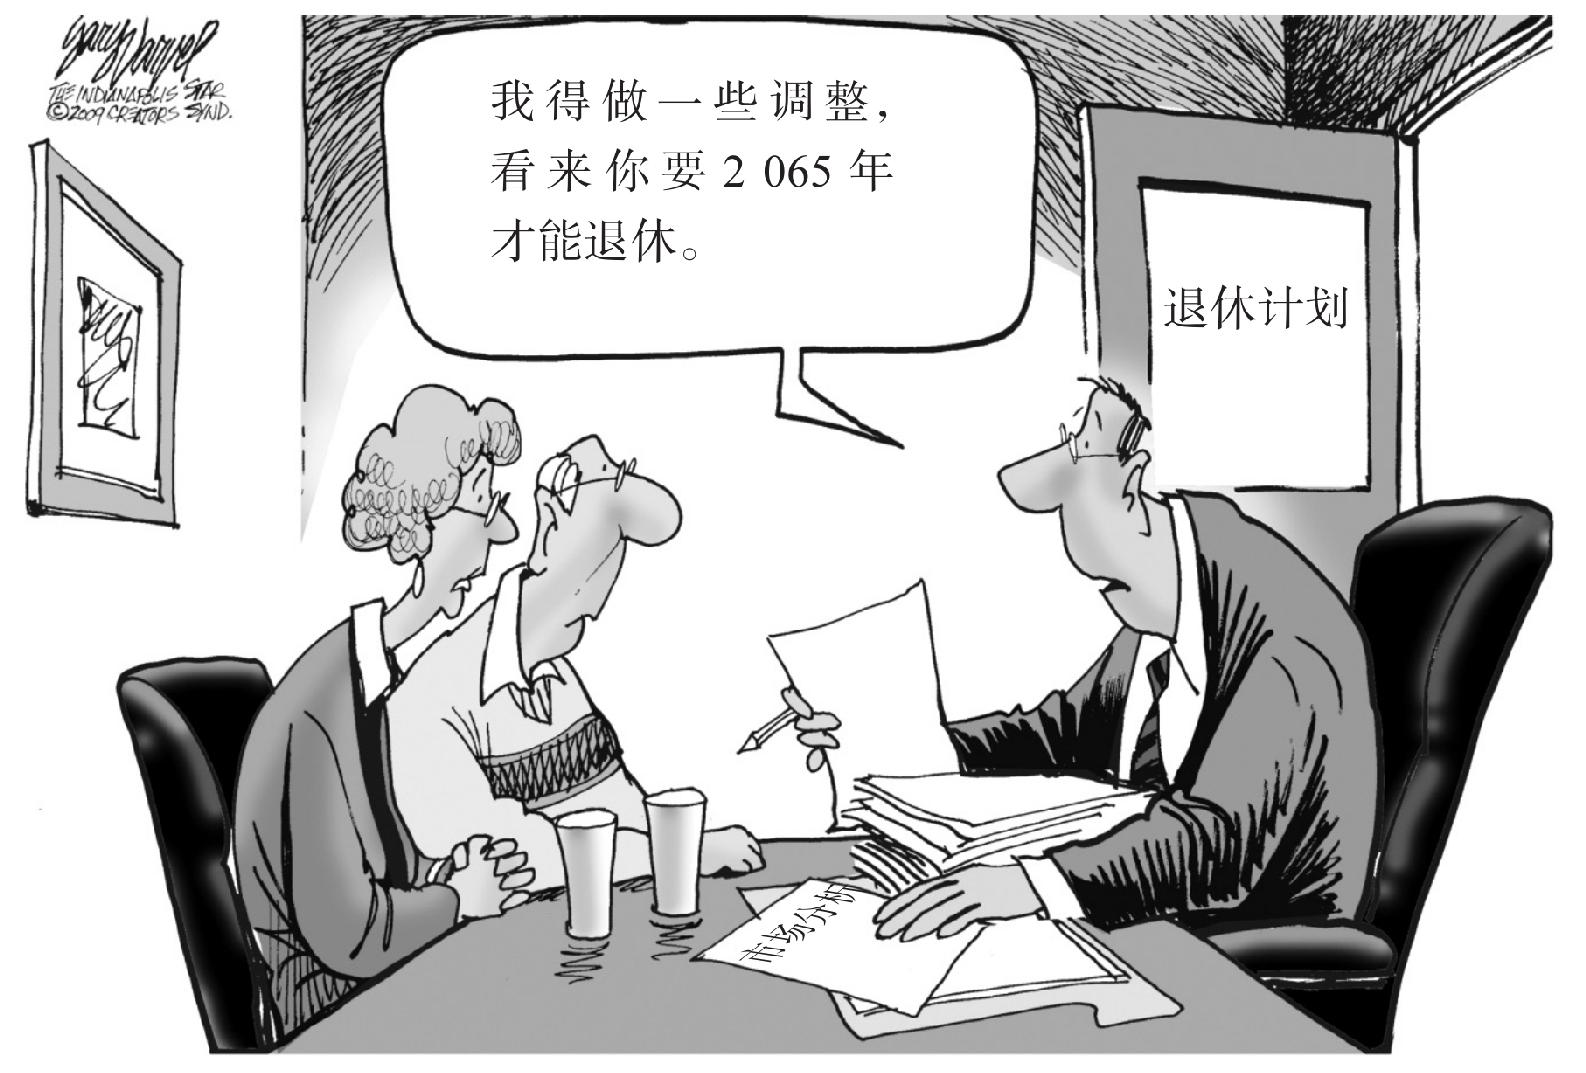
\includegraphics[width=0.78\linewidth,keepaspectratio]{image/15-4.jpg}
\caption{}\label{fig:15-4}
\end{figure}

\subsection{第五大梦想：绝对财务自由}

绝对财务自由是什么样的？是不是说你可以想做什么就做什么，什么时候想做就能什么时候做？如果你和你的家庭再也不用特别想得到什么东西了，那会是什么样的感觉？你想得到的都得到了，如果你能够不求回报地给予别人，完全按照自己想要的方式生活，而不是别人想要的方式，而且根本不用你再去靠工作来赚钱维持，你睡觉也照样能赚钱，这些钱就是你的投资收益，它会为你提供没有限制的生活方式。也许，你愿意给你的父母买一套房子，他们梦想有自己的房子好多年了；也许，你想设立一个慈善基金来为那些饥饿的人提供食物，或者帮助清理海洋。大胆设想，你实现绝对财务自由梦想之后能干什么。

我让罗恩和米歇尔告诉我，他俩能够想到的最大的梦想是什么。绝对财务自由对于他们来说是什么样子？米歇尔告诉我，她最大的梦想是买一个农场，把它变成一个教堂的营地。这要花多少钱？罗恩估计，买下农场要花200万美元，还要再投入100万美元进行维修，我又被他俩深深地打动了。

我可以看到在梳理这些数字的时候，他们发自内心的激动。

如果借钱购买这个牧场，他们每年需要大概12万美元还本付息（300万美元，每年要付4\%的利息）。这完全在他们的能力范围之内！

他们还有别的梦想吗？罗恩喜欢冒险和旅行，拥有私人飞机是他的终极梦想。于是，我引导他做了一个练习，这个练习我也让那个想成为10亿美元富豪的小伙子做过，我让他相信租一架飞机可以给他带来同样的便利和满足，和他自己拥有和保养一架私人飞机的巨额费用相比，租金是相当低的。你明白我的意思了吗？你并不需要拥有私人飞机，也能享受到像自己拥有私人飞机那样的生活方式。你并不是非得买一支球队才能坐在包厢里看球，你并不需要花钱买下整支球队来成为一个球队的所有人——你可以成为股东之一，同样能享受所有的特权。我的朋友魔术师约翰逊就是这么做的，他和收购了洛杉矶道奇队的彼得·古伯，还有其他几个古根海姆棒球管理公司的合伙人参加了一个财团。他们花了21.5亿美元得到了球队和球场。我可以向你保证，魔术师约翰逊并没有投入21.5亿美元，但是他得到的快乐、骄傲、激动、影响力、乐趣，和他一个人全部拥有所有股权是一样的。

这种想法创造出你想要的生活品质，让你和你所爱的人享受到想要的幸福生活。大多数人只是做梦，而有些人能活出梦想的生活。为什么人和人之间的差别这么大？因为大多数人只是做梦，却从来没有算清楚他们梦想的价码是多少。他们想象出来的数字简直太大了，连自己都不敢相信，难怪他们从未开始走上实现梦想的旅程。没有一个梦想是你不能实现的，只要你全力投入，足够有创意，愿意找出一种方式，给别人的生活增加更多的价值，你就比其他任何人增加的价值都多。

现在，你也能看出来对于大多数人来说，绝对财务自由这个类型的梦想主要是为了乐趣。在我举办的研讨会上，我只给少数人做这个练习，这些人确实有非常大的梦想，而且知道这些梦想的价码。我明白，大多数人从来不会获得绝对的财务自由，去梦想，去释放你的欲望，这能产生力量，有时这种能量非常强大，可能会激发你去实现梦想，让你想去赚更多的钱，帮助你去更快地达到你的目标。但是还有另外一个原因，你也许根本不用工作就能获得财务安全，然后再利用部分时间做一些你喜欢做的事情，你可以实现更高一层的梦想——财务独立。或者你已经获得财务独立了，然后通过投资收益和部分时间工作，用这部分多出来的收入，你可以实现更高一层的梦想，体验到财务自由的奢侈享受。

所以大胆地梦想你实现绝对自由之后想做的事情吧！写下你的终极梦想清单。你永远不会知道，如果你的愿望真的完全被释放了，你能创造出什么。

下面我们来看看罗恩计算出的自己实现绝对财务自由所需要的收入：

1.买一个牧场作为教堂营地所需要的费用为300万美元，贷款利率是4\%：每个月还款1万美元

2.比奇公司的一架私人飞机，购买它需要30万美元，贷款利率是5\%：每个月需要支付3181美元

3.实现财务自由需要的月收入水平是：每月42910美元

4.实现绝对财务自由的月收入水平是：每月56091美元

5.现在把上面的月收入乘以12，你就会得到实现绝对财务自由的年收入水平：每年673092美元

购买一艘20英尺长的钓鱼船，每年给教堂捐款10万美元，购买一个滑雪度假公寓、一架私人飞机、把农场改造成一个教堂的营地，再加上他们维持现有的生活方式，而且不用去工作，达成以上所有项目，罗恩和米歇尔每年收入需要达到673092美元。把它乘以20，他们需要达到的财富规模是1350万美元。他们原来设想只是获得财务安全和财务独立就需要2000万美元，与此相比，这个数字要少1/3。

你的数字是多少呢？

1.奢侈品1：\_\_\_\_美元/月

2.奢侈品2：\_\_\_\_美元/月

3.奢侈品3：\_\_\_\_美元/月

4.实现财务自由所必需的月收入：\_\_\_\_美元/月

5.实现绝对财务自由所必需的月收入总额：\_\_\_\_美元/月

6.把上面的月收入乘12，你就可以算出来你的绝对财务自由所必需的年收入：\_\_\_\_美元/月

\begin{BookQuote}
只有一件事能够让梦想不可能实现：害怕失败。

\hfill ——保罗·科埃略
\end{BookQuote}

你写下来的所有这些数字，你自己看起来感觉怎么样呢？我希望你已经看到了你的财务梦想的价码，它比你原来想象的要小很多。你现在已经选出来三个梦想作为目标去努力追求，其中至少包括一个短期目标和一个长期目标。这些梦想中哪一个是你“三生万物”的梦想？对于那些想要达到更高层次梦想的人来说，“三生万物”梦想是财务安全、财务独立、财务自由。你如果还没有做好，选择三个，把它们写下来。

如果你是一个婴儿潮时代出生的人，经历2008年的金融危机后，日子过得很艰难，这五个梦想里哪一个对于你来说是绝对必须要实现的？财务安全，是吗？这里有个好消息：你也许并没有用很多时间把你的储蓄和投资积累到一个关键的规模，但是你绝对可以拥有财务安全，我会展示给你看。也许你永远不会达到财务独立，但如果你把财务独立当成“必须的”，你就能达到了。如果你人生刚刚起步，还很年轻，那么你的路还长着呢。你可以实现财务自由，甚至是绝对财务自由，对这么大的梦想心里也没有什么压力。但关键是，要决定什么对于你来说是最重要的，知道你要实现这个财务梦想所需要的收入数字是多少。为什么？因为再过一会儿，我们就要进入本书的下一章，你就能计算出来，你还需要多少年才能实现这些梦想，年数计算基于一个合理的平均年收益率水平，以及你现在每年能够积累多少钱。然后我们会制订一个规划去达到这个目标。养兵千日，用兵一时。决战的时候到了。我会引导着你一步一步地走下去，每件事都设计好，完全可以自动操作。至关重要的是你要一直保持不断前进。

我希望你能感觉内心充满力量，激动兴奋，因为你正在通向财务自由的大道上。

我希望你知道，你是你的人生的创造者，而不仅是管理者。有时我们忘了，我们过去的人生已经创造出了多少。我不用问你是谁，我就知道你人生现在的样子就是你过去的梦想，或者是过去的目标，甚至可能是过去看起来好像根本不可能达到的状态。它可能是你想要得到的一份工作，或者是你想要得到的一个更高层次的位置，或者是你做梦都想要的一辆车，或者是你非常想去看的一个地方。也许，那个地方后来你不但看了，而且现在还住在了那个梦想的地方。也许某个人，你以前觉得自己绝对高攀不上，连一起出去都不可能，但现在你们结婚了。如果是这样的话，赶紧过去，给他一个吻。别忘了，这种亲密关系过去看起来根本不可能，但你创造出来了，你把梦想变成了现实。

今天，你生活中的什么东西曾经是你过去的梦想？过去你有过什么渴望，当时看起来非常难以实现，甚至觉得根本不可能实现，但是现在成了你生活的一小部分？你如果想记起来，你是你的生活的创造者，而不仅是你现在生活环境的管理者，首先你必须重新联系上你过去有意识地创造出来的那些事情。花些时间，记下来三四件这样的事情。你要注意，你列出来的清单并不需要都是你的伟大成就，有的时候反而是一些小事看起来很难，或者根本不可能实现，但等你做到了，实现了，它们能给我们提供重要的经验教训，指导我们如何实现和完成更大的目标。现在你的生活中也许有时会有某些东西，曾经看起来非常困难或者不可能实现，但现在你都拥有了。不过，现在你对这些东西都司空见惯了，觉得是理所当然、自己应该拥有的。熟悉定律说：如果我们一直待在任何一个东西（或任何一个人）周围，时间一长，我们就会觉得这些东西、这些人是理所当然的。所以重新唤醒自己，欣赏自己过去把梦想变成现实的成就，一个一个地记下来，它们就是你的历史成就清单。

第二，如果你需要重新评估一下，你采取了哪些步骤，把你的梦想变成了现实。现在就花些时间来做，从你实现的梦想里选出一个。当初，你的第一个行动是什么？把这些行动步骤一一记下来。

毫不夸张地说，我问过成千上万的人，他们是如何把某些曾经看起来不可能的事变成自己生活里的一部分的？他们是如何从梦想中创造出现实的？这个过程我们都要经历，一般分成三步。

第一步，释放你的饥渴和欲望，唤醒像激光一般的专注力。有些事情发生在你的内在：你受到某种事情的激发，让你如此兴奋激动，以至你的渴望完全被释放出来了——你变得对这件事疯狂地着迷，你专注在你渴望的目标上，像激光一般专注！你的想象力被点燃了。或者你撞到了天花板，达到了临界点，或者触动你内心的某个地方，确认你再也不满足于过着这样的生活了。你做出决定，再也不要回到过去了。你开始极其强烈地专注于追求新生活，或者你渴望得到新东西，这可能是换个工作，离婚了，改变了生活方式。你释放出你对目标的渴望——你的焦点换到哪里，能量就会流到哪里。

你是不是有过这种体验？你买了一套很贵的衣服，突然之间你发现很多人穿这套衣服，或者你买了一辆汽车，突然你看到很多人开这款汽车呢？这种事是怎么发生的？因为你大脑的一部分潜意识，被称为网状激活系统，知道这事现在是重要的了，于是它开始注意到所有和这件事相关的东西。这款车、这款礼服其实一直在你身边，而且经常出现，只是你一直没有注意到，但是你现在开始注意到了，因为你的潜意识让你意识到了这些东西，而你以前只是看，却没有看见。

这也是你读本书时会体验到的，你开始注意到公募基金的收费，开始注意到资产配置这个听起来很专业的词。你开始听到一些你以前从来没有听说过的东西：高频交易、基金定投……它们对于你来说开始活跃起来，到处都是。因为你的大脑现在知道，这些东西是很重要的。重要的东西、受到关注的东西，能量就会流向它们。当你拥有了这种饥渴、渴望、专注后，第二步就开始启动了。

第二步，采取大量的而且有效的行动。如果你的渴望真正被释放出来了，你非常痴迷地专注于你想得到的，你就会受到召唤去做任何需要做的事情，来让你的梦想成真。你拥有的能量和灵活性是没有限制的，你会想尽一切办法追求你想要得到的东西。在你的心中，你知道大量的行动是包治百病的万能灵药。如果愿意付诸行动和努力，你就能够到达目的地。你以前这样做到过，对吧？也许，曾经有一段时间，你必须去看你心爱的女孩，于是你借了辆车，通宵开车，穿越暴风雪，去她读的大学见她。也许你动用了所有的关系，搞得天翻地覆，就是想把你的孩子送进最好的学校，以满足孩子的需要。如果是“必须的”，而不只是“应该的”，你肯定会找到方法做成的。

但是在这里我要给你一个警告，在所有这些努力的背后，你需要做出有效的行动，对不对？你可以付出你所有的努力来为你的未来做储蓄。但是，把你所有的钱投到一个私立的账户里面，那里都是收费很高、业绩糟糕的公募基金，那么你根本不会赚到多少钱，你的退休生活肯定不好。或者你可以用所有的钱投资一家公司，然后眼看股票一天暴跌了40\%。所以尽管你愿意做你需要做的任何事，但是你还是必须小心谨慎地执行计划，因为你必须努力、有效地执行，才能够创造出魔法般的神奇效果。本书就是你的地图、你的财务蓝图。通过持续采取大量有效的行动，你可以不断地修正自己的路径，当它不再有效的时候，你采用或尝试一些新的路径，就会不断地前进，接近你的梦想，但是最后一个因素扮演着非常重要的角色，它决定了你的梦想能否成真。

第三步，恩惠！有些人称之为运气、巧合、命运、上帝之手。我称之为恩惠：承认在这个世界上有很多事超出了我们的控制。也许有更高层次的力量，既给了我们独一无二的生命特权，也给了我们洞察和指引的天赋，我们对此敞开心扉，就可以得到它们。当你决定了前两步如何走，上帝或者宇宙或者恩惠，不管你如何称呼，都会介入，支持你做的事情，这是多么令人震惊啊。首先你把你自己该做的那一部分事情做好，剩下所有的好事都会涌向你。我们都有过那种意外交上好运的经历。有些事情发生了，根本没法解释，所以我们称之为巧合。我们错过了一辆火车，结果碰到了一个人，后来我们结婚了。我们替朋友临时上几天班，结果这让我们找到了梦寐以求的工作。我们事先不知道会有这样的好事，也并没有凭本事努力争取——这种好事就自动发生了。对于我来说，这就是恩惠。你知道的越多，越感恩发生在你生命中的恩惠，你体验到的那份恩赐就越多，这些远远不是你自己的力量能够创造出来的。我的生命中已经发生很多次这样的好事了，我知道上天的恩惠是真实存在的。我也知道你内心那份感谢上天让自己能交上好运的心情。感恩的时候，心里就没有愤怒了；感恩的时候，心里就没有恐惧了。

那么，你准备好了吗，成为一个你自己生活的创造者，而不仅是你周围环境的管理者？你知道你做投资的真正目的吗？一份终身的收入！你的梦想成为你这个人的一部分，成了“必须的”，你大脑的潜意识日夜专注，你非把这事完成不可，你有这么疯狂和着迷吗？你是不是愿意做所需要做的事，让梦想成真？那么，翻开下一页，去做很多人没能做成的事。

现在是时候去做一个规划了……
